\documentclass[a4paper,12pt,italian,towside]{article}
\usepackage[latin1]{inputenc}
% Comment the following line to deny the usage of umlauts and other non-ASCII characters
%\usepackage[italian]{babel}

%pack per link
\usepackage{hyperref}
\hypersetup{colorlinks=true,linkcolor=blue}

%pack per colori
\usepackage{xcolor}
\usepackage{xcolor,listings}

%pack tabelle
\usepackage{graphicx}



\setcounter{tocdepth}{3}


%intestazioni e pie pagina
\usepackage{fancyhdr}
\pagestyle{fancy}
\chead{}
\cfoot{\thepage}
\lhead{}
\renewcommand{\headrulewidth}{0.4pt}

%Formattazione per codice SQL
\usepackage{textcomp}
\usepackage{color}

\definecolor{codegreen}{rgb}{0,0.6,0}
\definecolor{codegray}{rgb}{0.5,0.5,0.5}
\definecolor{codepurple}{HTML}{C42043}
\definecolor{codeblue}{HTML}{0000FF}
\definecolor{backcolour}{HTML}{F2F2F2}
\definecolor{bookColor}{cmyk}{0,0,0,0.90}  
\color{bookColor}

\lstset{upquote=true}

\lstdefinestyle{mystyle}{  
	commentstyle=\color{codegreen},
	keywordstyle=\color{codeblue},
	numberstyle=\footnotesize\color{codegray},
	stringstyle=\color{codepurple},
	basicstyle=\footnotesize,
	breakatwhitespace=false,         
	breaklines=true,                 
	captionpos=b,                    
	keepspaces=true,                                   
	numbersep=-10pt,                  
	showspaces=false,                
	showstringspaces=false,
	showtabs=false,      
}
\lstset{style=mystyle} 


%*************************************************************************%
% Start the document
\begin{document}



\begin{titlepage}
	\centering
	
\includegraphics[scale= 0.2]{unipd.png} \centering 
	{\huge \\ \medskip Progettazione Base di Dati: \\ Data Base dei Corsi di studio UniPd\\ \medskip \medskip  \medskip \normalsize Francesco Pham, Luca Moroldo, Piero Soravia, Giovanni Sissa \\ \medskip 28/3/2019\par }
	

\end{titlepage}



\newpage

%indice
\tableofcontents

\newpage
% *****sezione1*****
\section{Descrizione del progetto}
Si vuole realizzare una base di dati per modellare correttamente i Corsi di Laurea dell'Universit\'a di Padova.
Si vogliono rappresentare tutti i dati funzionali ai Corsi di Laurea come Scuole, Classi, Curriculum, Attivit\'a formative e relativi SSD, Coorti, Percorsi e Docenti.
In questo progetto non vengono coinvolti studenti o piani di studio.
\par
La modellazione viene fatta coerentemente al sito  \href{https://didattica.unipd.it/}{didattica.unipd.it}, fonte partanto del minimondo di interesse.



\subsection{Requisiti strutturati}

\hspace{0.6cm}\textbf{Scuola}\\
Le Scuole hanno funzioni di coordinamento e di razionalizzazione delle attivit\'a didattiche, compresa la proposta di istituzione, attivazione, modifica, disattivazione o soppressione di corsi di laurea, nonch\'e di gestione dei servizi comuni. Ogni Scuola pu\'o attivare diversi corsi di laurea in linea con il settore accademico di interesse. Ad ogni Scuola \'e assegnato un codice a livello Universitario.
\newline

\textbf{Classe}\\
Le Classi sono dei contenitori che raggruppano i Corsi di Laurea dello stesso ciclo, comunque denominati dagli Atenei, aventi gli stessi obiettivi formativi qualificanti e attivit\'a formative attivate per un numero di crediti e in settori individuati come indispensabili. Le caratteristiche delle Classi sono fissate a livello nazionale, con appositi Decreti Ministeriali e identificate da codici, e sono quindi comuni a tutti gli atenei. I corsi di laurea appartenenti alla stessa Classe hanno identico valore legale.
\\

\textbf{Corso di Laurea}\\
I Corsi di Laurea sono l'insieme di tutte le attivit\'a formative, obbligatorie e non, proposte da un ateneo per conseguire la laurea. La laurea rilasciata \'e coerente al Corso di Laurea scelto. I Corsi di Laurea sono inquadrati in Classi ministeriali, possono prvedere pi\'u percorsi e afferiscono a una scuola. Per il conseguimento della Laurea, e quindi il completamento del relativo corso, lo studente deve conseguire un numero prefissato di CFU (180 per le lauree triennali). Ogni corso di Laurea appartiene ad un ordinamento legislativo che ne definisce la struttura e la validit\'a legale. Ogni Corso di Laurea pu\'o avere, a discrezione della Scuola, pi\'u Curricula. Ogni Ateneo identifica un Corso di Laurea con un codice univoco.\\


\textbf{Curriculum}\\
Un Curriculum \'e una denominazione di un Corso di Laurea che ne definisce gli obbiettivi oltre che a differenziare lo stesso in un insieme di attivit\'a formative differenti. Pi\'u studenti possono dunque conseguire la stessa laurea con percorsi alternativi a seconda dei loro interessi e attitudini scegliendo, ad esempio, un Curriculum Generale piuttosto che un Curriculum Applicativo.
Ogni Ateneo identifica un Curriculum con un codice univoco.\\


\textbf{Attivit\'a Formativa}\\
Le Attivit\'a Formative sono il cuore di un Corso di Laure e rappresentano tutti gli step che uno studente deve superare per conseguire la Laurea. Le Attivit\'a formative possono essere di quattro tipi: Tirocinio, Lingua, Prova Finale e Insegnamento. Ogni attivit\'a? formativa si inserisce in un Corso di Laurea in un anno (I, II, II IV o V a seconda del tipo di Laurea) e in un semestre ( I o II). Ogni Attivit\'a Formativa \'e riferita a un Docente responsabile che ha il compito di definirla in termini di: tipo di valutazione, prerequisiti, conoscenze e abilit\'a da acquisire, modalit\'a di esame, criterio di valutazione, contenuti, attivit\'a, materiali, testi consigliati e lingua di emissione. Ogni Attivit\'a formativa si riferisce poi a un Dipartimento some sede fisica delle lezioni. Infine ogni Attivit\'a formativa \'e legata a uno o pi\'u SSD dai quali, al conseguimento da parte dello studente dell' esame, vengono rilasciati CFU. Le Attivit\'a Formative sono soggette a vincoli, decisi dalla Scuola, in termini di superamento di altre Attivit\'a formative precedenti. All'interno di ogni ateneo le Attivit\'a formative sono identificate da un codice.\\

\textbf{Docente}\\
I Docenti sono gli attuatori di un Attivit\'a Formativa. Pi\'u Docenti possono essere coinvolti in una stessa Attivit\'a Formativa con ruoli differenti. Dei Docenti coinvolti in un Attivit\'a, uno e uno solo \'e il Responsabile della stessa e ha il compito di definirla come descritto dal paragrafo Attivit\'a formativa. Dei docenti si vogliono poi poter conoscere tutti i dati relativi ai contatti e agli ambiti di ricerca. Ogni docente pu\'o partecipare a pi\'u attivit\'a formative. Ogni Docente ha una matricola identificativa assegnata dall'Ateneo.\\


\newpage
\subsection{Operazioni sulla basi di dati}
Vengono presentate le seguenti operazioni esemplificative della capacit\'a espressiva della base di dati.
% Please add the following required packages to your document preamble:
% \usepackage{graphicx}
\begin{table}[!h]
	\resizebox{\textwidth}{!}{%
		\begin{tabular}{ll}
			\textbf{Operazione} & \textbf{Tipo} \\ \hline
			Dati un Corso di Studi e una Coorte trovare tutte le Attivit� Formative ordinate per anno e semestre. & Interrogazione \\ \hline
			\begin{tabular}[c]{@{}l@{}}Dati un Corso di Studi e una Coorte trovare tutte le Attivit� Formative ordinate per anno e semestre,\\ mostrare canale, anno accademico, nome e cognome del docente se il corso � attivato.\end{tabular} & Interrogazione \\ \hline
			\begin{tabular}[c]{@{}l@{}}Dati il codice di una Attivit� Formativa, il canale, l'anno accademico e il responsabile trovare i \\ dettagli dell'Attivit� Formativa.\end{tabular} & Interrogazione \\ \hline
			Mostrare tutti i Corsi attivati con il relativo Codice, Nome, Anno Accademico, Canale e Responsabile. & Interrogazione \\ \hline
			Dati una Scuola e un tipo (LT/LM/CU) elencare i Corsi di Laurea. & Interrogazione \\  \hline
			\begin{tabular}[c]{@{}l@{}}Dati un Curriculum, un Corso di Laurea e una Coorte mostrare la somma dei crediti delle Attivit� \\ Formative divisi per SSD.\end{tabular} & Interrogazione \\ \hline
			Dati due Corsi di Laurea e una Coorte mostrare le Attivit� Formative non in comune tra i due Corsi. & Interrogazione \\ \hline
			Inserimento di un nuovo Curriculum. & Modifica \\ \hline
			Inserimento di un nuovo Corso di Laurea. & Modifica \\ \hline
			Inserimento di una nova Coorte. & Modifica \\ \hline
			Inserimento di una nuova Attivit� Fomrativa. & Modifica \\ \hline
			Inserimento di un Docente. & Modifica \\ \hline
		\end{tabular}%
	}
\end{table}


\subsection{Glossario}
\begin{table}[!h] %!h forza la figura sotto il titolo
	\resizebox{\textwidth}{!}{%
		\begin{tabular}{llll}
			
			\multicolumn{1}{c}{\textbf{Termine}} & \multicolumn{1}{c}{\textbf{Descrizione}} & \multicolumn{1}{c}{\textbf{Sinonimi}} & \multicolumn{1}{c}{\textbf{Collegamenti}} \\ \hline \hline
			Corso di  Laurea & \begin{tabular}[c]{@{}l@{}}Insieme di tutte le Attivita Formative\\ necessarie a Laurearsi.\end{tabular} & Corso di studi. & \begin{tabular}[c]{@{}l@{}}Scuola, Classe, \\ Attivit� Formativa, \\ Curriculum.\end{tabular} \\ \hline
			\begin{tabular}[c]{@{}l@{}}Istanza Attivit� \\ Formativa\end{tabular} & \begin{tabular}[c]{@{}l@{}}Insegnamento, Prova finale, Tirocinio o \\ Lingua che uno studente trover� effetti-\\ vamente nel suo piando si studi.\end{tabular} & Esame, Corso. & \begin{tabular}[c]{@{}l@{}}Docente, Percorso,\\ Attivit� Formativa\end{tabular} \\ \hline
			Responsabile & \begin{tabular}[c]{@{}l@{}}Docente incaricato di istanziare un'At-\\ tivit� Formativa e responsabile di tale \\ Attivit� per quell'anno.\end{tabular} & \multicolumn{1}{c}{-} & \begin{tabular}[c]{@{}l@{}}Atttivit� Formativa,\\ Istanza Attivit� \\ Formativa, Ruolo\end{tabular} \\ \hline
			Coorte & \begin{tabular}[c]{@{}l@{}}Insieme di studenti immatricolatisi nel \\ medesimo anno. Riferendosi a Coorte\\ come anno si identifica il momento di \\ schedulazione di tutti le Attivit� che\\ gli studenti di quella Coorte vedranno \\ proposte durante la propria carriera.\end{tabular} & Anno, Classe. & \begin{tabular}[c]{@{}l@{}}Attivit� Formativa,\\ Percorso, Corso di\\ Laurea.\end{tabular} \\ \hline
			SSD & \begin{tabular}[c]{@{}l@{}}Settore Scientifico Disciplinare:\\ Distinzione disciplinare utilizzata nell'\\ Universit� in Italia per organizzare l'is-\\ truzione superiore.\end{tabular} & \multicolumn{1}{c}{-} & \begin{tabular}[c]{@{}l@{}}Attivit� Formativa,\\ CFU.\end{tabular} \\ \hline
			CFU & \begin{tabular}[c]{@{}l@{}}Credito Formativo Universitario:\\ modalit� utilizzata nelle Universit� ita-\\ liane per misurare il carico di lavoro \\ richiesto allo studente.\end{tabular} & Crediti. & \begin{tabular}[c]{@{}l@{}}SSD, Percorso,\\ Attivit� Formativa\end{tabular} \\ \hline
			Percorso & \begin{tabular}[c]{@{}l@{}}Istanza del Corso di Laurea relativa ad\\ un dato Curriculum e a una Coorte.\end{tabular} & Indirizzo. & \begin{tabular}[c]{@{}l@{}}Attivit� Formativa,\\ Curriculum Corso \\ di Laurea, Coorte.\end{tabular} \\ \hline
		\end{tabular}%
	}
\end{table}


\newpage
\clearpage
% *****sezione2*****
\section{Progettazione concettuale}

\subsection{Modello concettuale: Entit\`a-Associazione (E-R)}
Di seguito lo schema concettuale prodotto per la rappresentazione della realt\`a di interesse:

\begin{figure}[!h] %!h forza la figura sotto il titolo
	\caption{Schema E-R completo}
	\begin{center}
		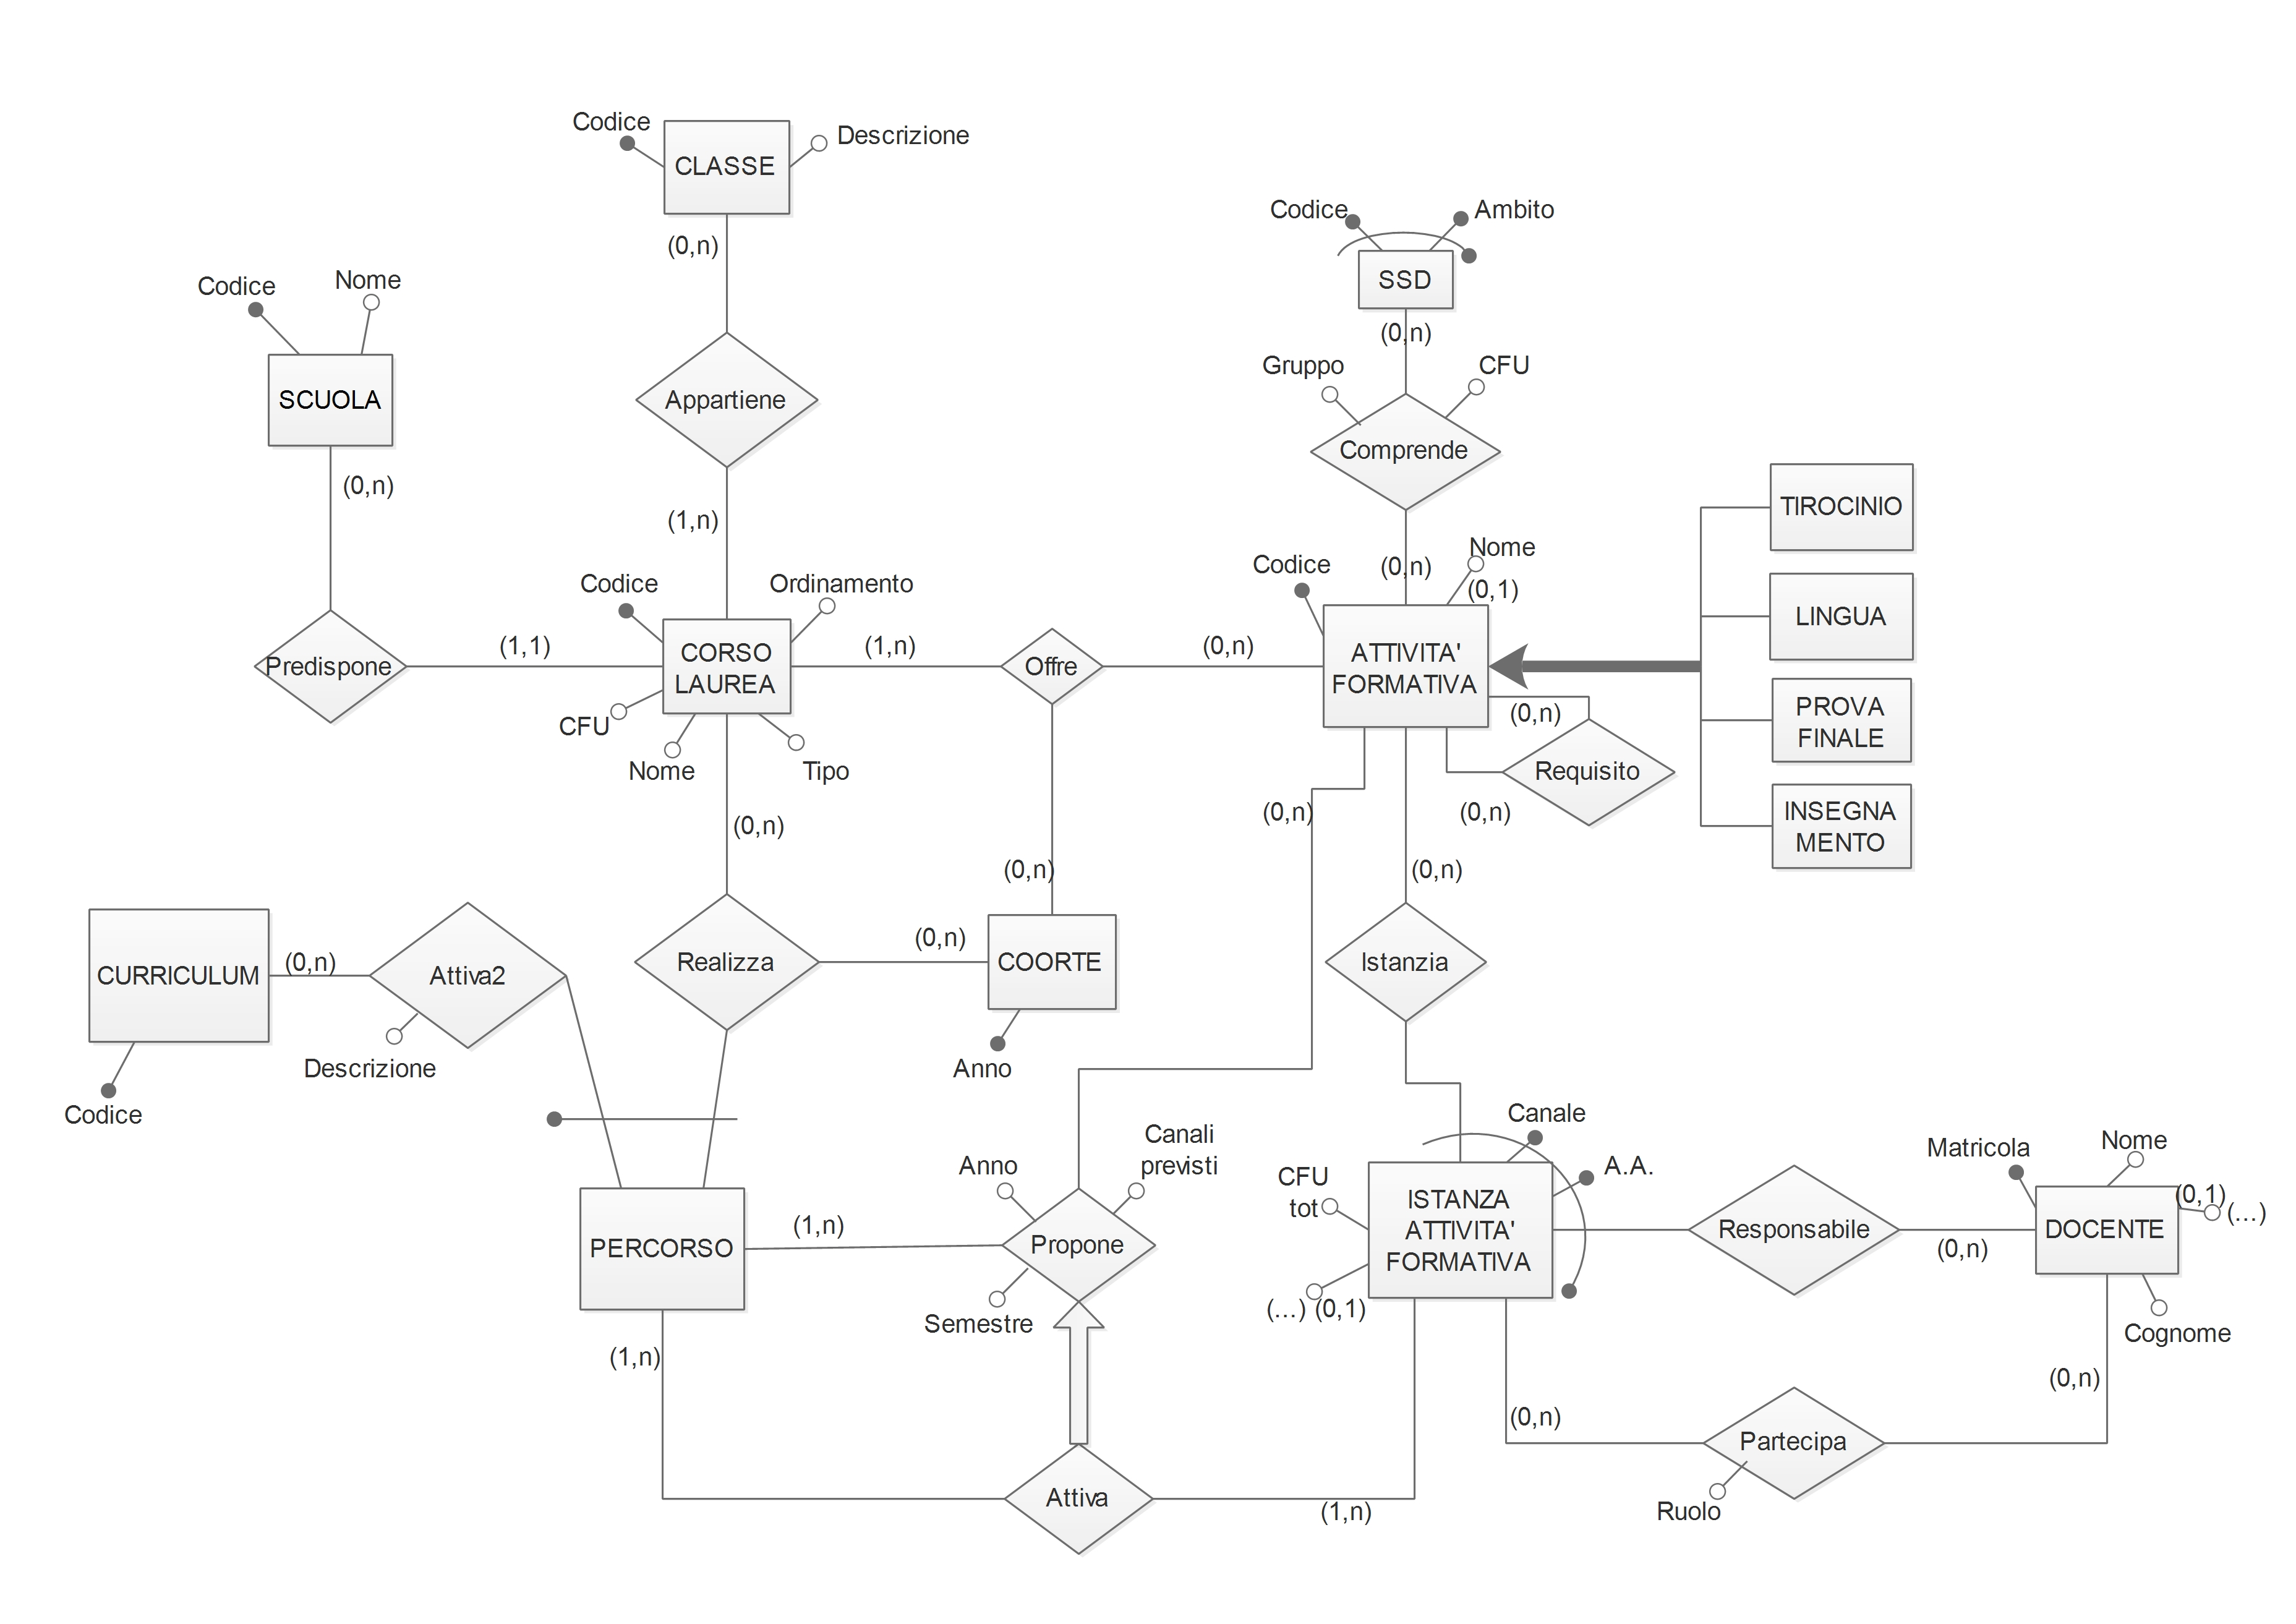
\includegraphics[scale=0.5,angle=90]{../Schemas/ER_diagram.jpg}
	\end{center}
\end{figure}

\subsection{Dizionario dei dati}

\subsubsection{Entit\`a}

\begin{table}[!h]
\resizebox{\textwidth}{!}{%
	\begin{tabular}{llll}
		
		\textbf{Entit�} & \textbf{Descrizione} & \textbf{Attributi} & \textbf{Identificatore} \\ \hline \hline
		Classe & Raggruppa Corsi di Laurea. & Codice, Descrizione. & Codice. \\ \hline
		SSD & Suddivide le Attivit�. & Codice, Ambito. &  Codice, Ambito. \\ \hline
		Attivit� Formativa & Attivit� Formativa ancora da istanziare. & Codice, Nome, Tipo insegnamento, CFU. & Codice. \\ \hline
		Coorte & \begin{tabular}[c]{@{}l@{}}Dato un Corso di Laurea offre Attivit� \\ Formative e le istanzia.\end{tabular} & Anno. & Anno. \\ \hline
		Curriculum & Specializza Corso di Laurea. & Codice, Nome. & Codice. \\ \hline
		Docente & \begin{tabular}[c]{@{}l@{}}Il responsabile del corso o un docente \\ che ne prende parte.\end{tabular} & \begin{tabular}[c]{@{}l@{}}Matricola, Cognome, Nome, Email, Diparti-\\ mento, Telefono, Qualifica, SSD, Ufficio, \\ Tesi, Aree di Ricerca, Curriculum, Pubblicazioni.\end{tabular} & Matricola. \\ \hline
		Scuola & Attiva Corsi di Laurea. & Codice, Nome. & Codice. \\ \hline
		Corso di Laurea & \begin{tabular}[c]{@{}l@{}}Offre Attivit� Formative, struttura gli \\ indirizzi.\end{tabular} & Codice, Nome, Scuola; Ordinamento & Codice \\ \hline
		Percorso & \begin{tabular}[c]{@{}l@{}}Istanza del Corso di Laurea relativa ad \\ un dato Curriculum e a una Coorte.\end{tabular} & Corso di Laurea, Curriculum, Coorte & \begin{tabular}[c]{@{}l@{}}Corso di Laurea, \\ Curriculum, \\ Coorte\end{tabular} \\ \hline
		\begin{tabular}[c]{@{}l@{}}Istanza Attivit�\\ Formativa\end{tabular} & \begin{tabular}[c]{@{}l@{}}Attivit� Formativa vera e propria che \\ gli studenti si troveranno proposta in \\ un dato semestre con relativo esame \\ che dovranno superare.\end{tabular} & \begin{tabular}[c]{@{}l@{}}Attivit� Formativa, Canale, Anno Accademico,\\  Responsabile, Tipo Valutazione, Dipartimento, \\ a Frequenza Obbligatoria, Corso Singolo, Corso \\ Libero, Prerequisiti, Acquisire, Modalit� Esame, \\ Criteri Valutazione, Contenuti, Attivit�, Materiali, \\ Testi, Lingua.\end{tabular} & \begin{tabular}[c]{@{}l@{}}Attivit� Formativa, Canale, Anno \\ Accademico, Responsabile.\end{tabular} \\ \hline
		&  &  &  \\
		&  &  &  \\
		&  &  &  \\
		&  &  & 
	\end{tabular}%
}
\end{table}

\subsubsection{Associazioni}

% Please add the following required packages to your document preamble:
% \usepackage{graphicx}
\begin{table}[!h]
	\resizebox{\textwidth}{!}{%
		\begin{tabular}{lll}
			\textbf{Associazione} & \textbf{Attributi} & \textbf{Entit� collegate} \\ \hline \hline
			Attiva &  & Istanza Attivit� formativa (1,N), Percorso(1,N). \\ \hline
			Comprende & CFU, Gruppo. & Attivit� Formativa (0,N), SSD (0,N). \\ \hline
			Requisito &  & \begin{tabular}[c]{@{}l@{}}Attivit� formativa {[}richiesta{]} (0,N), \\ Attivit� formativa {[}richiede{]} (0,N).\end{tabular} \\ \hline
			Responsabile &  & Istanza Attivit� Formativa (1,1), Docente (0,N). \\ \hline
			Partecipa & Ruolo. & Docente (0,N), Istanza Attivit� Formativa(0,N). \\ \hline
			Appartiene &  & Corso di Laurea (1,N), Classe (0,N). \\ \hline
			Offre &  & \begin{tabular}[c]{@{}l@{}}Corso di Laurea (1,N),  Attivit� formativa (0,N),\\ Coorte (0,N).\end{tabular} \\ \hline
			Predispone &  & Scuola (0,N), Corso di Laurea (1,1). \\ \hline
			Realizza &  & Corso di Laurea (0,N), Coorte (0,N), Percorso (1,1). \\ \hline
			Attiva2 &  & Curriculum (0,N), Percorso (1,1). \\ \hline
			Propone & \begin{tabular}[c]{@{}l@{}}Semestre, Anno, \\ Canali Previsti.\end{tabular} & Percorso (1,N) Attivit� Formativa (0,N). \\ \hline
			Istanzia &  & Attivit� Formativa (0,N), Istanza Attivit� formativa (1,1). \\ \hline
		\end{tabular}%
	}
\end{table}

\subsection{Schema concettuale, regole di vincolo}

\'E necessario definire alcune regole di vincolo per una corretta rappresentazione della realt\'a? di interesse:
\begin{itemize}
	\item RV1: i CFU assegnati ad un Corso di Laurea devono essere minori della somma dei CFU delle Attivit\'a Formative proposte dai Percorsi che realizzano il corso di laurea.
	\item RV2: i CFU totali assegnati ad una Attivit\'a Formativa devono essere pari alla somma dei CFU assegnati agli SSD che compongono l'Attivit\'a Formativa.
	\item RV3: la somma dei CFU delle Attivit\'a Formative offerte per un Corso di Laurea deve essere maggiore dei CFU richiesti dal Corso di Laurea per ogni Coorte.
	\item RV4: le Attivit\'a Formative proposte da un Percorso per una Coorte devono essere offerte dal relativo Corso di Laurea per la stessa Coorte.
	\item RV5: le istanze attivate per un Percorso devono essere proposte dallo stesso. 
	\item RV6: le Istanze delle Attivit\'a Formative attivate per un Percorso devono svolgersi in un anno accademico uguale o maggiore all'anno della Coorte associata al Percorso sommato all'anno in cui l'Attivit\'a? Formativa \'e prevista.
	\item RV7: gli Insegnamenti devono avere almeno un SSD e dei Crediti.
\end{itemize}

\newpage
% *****sezione3****
\section{Progettazione logica}

\subsection{Ristrutturazione schema E-R}

\begin{figure} [!h] %!h forza la figura sotto il titolo
	\caption{Schema E-R completo}
	\begin{center}
		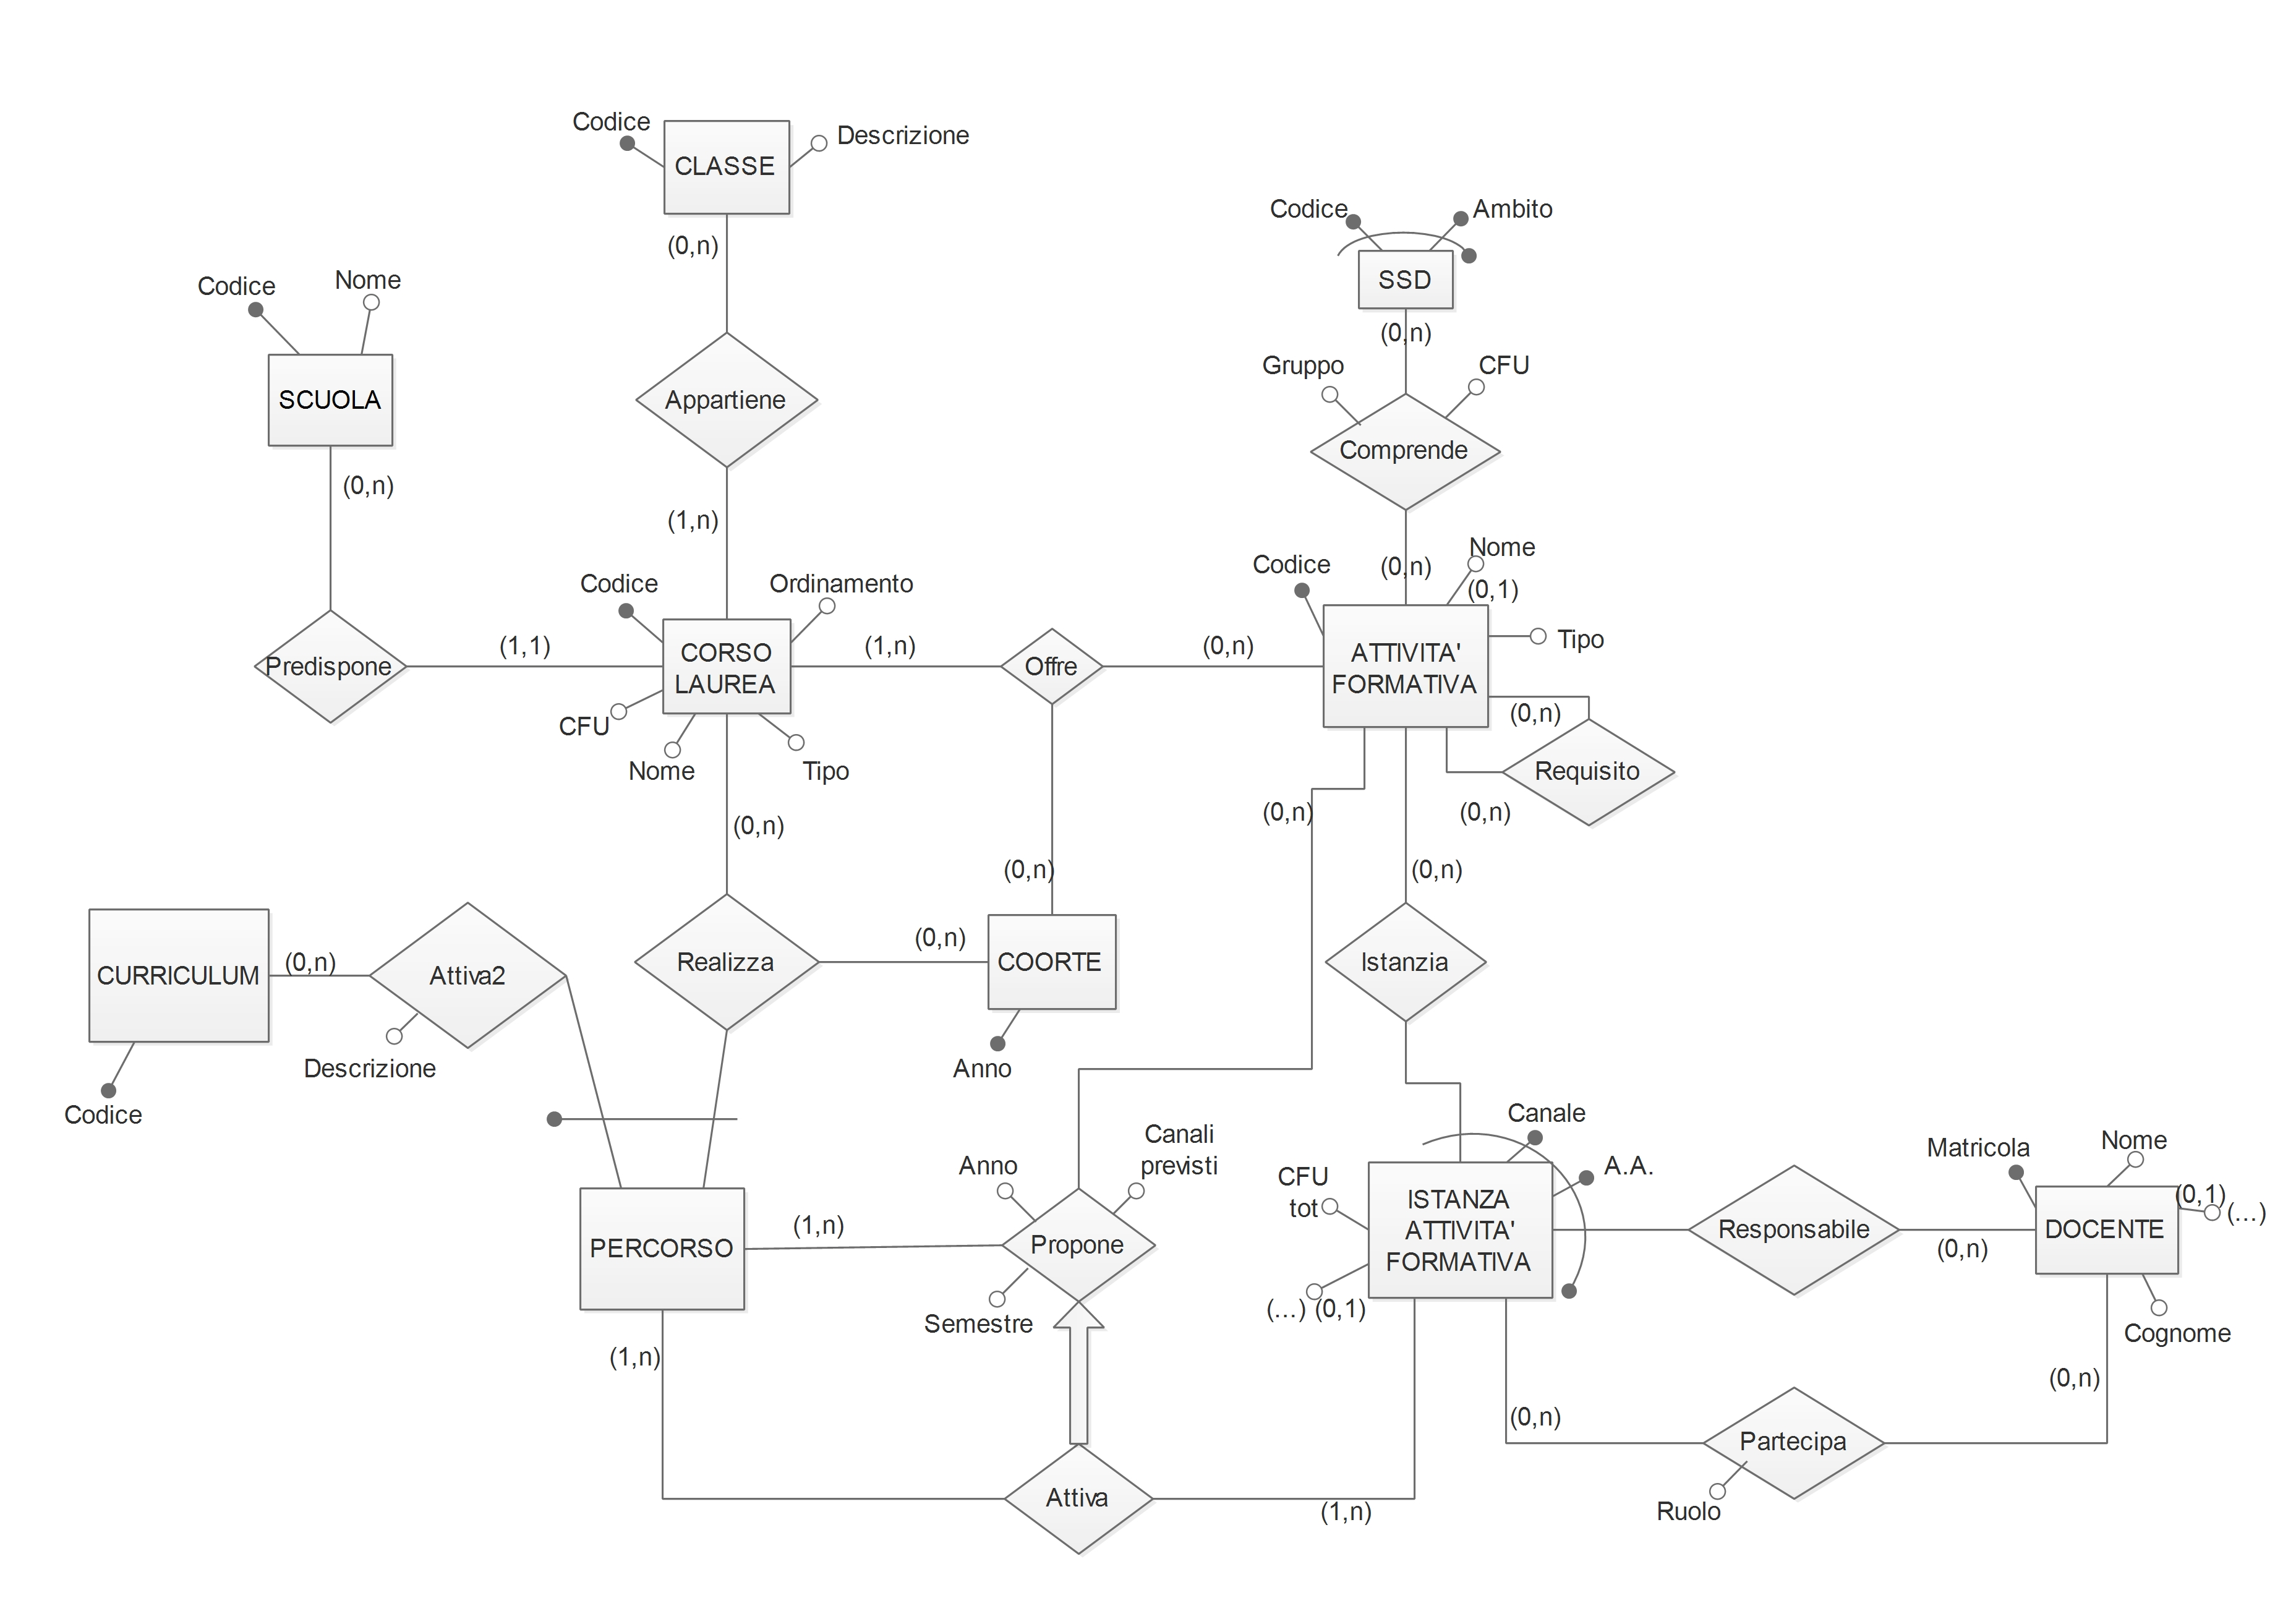
\includegraphics[scale=0.455,angle=90]{../Schemas/ER_diagram_restructured.jpg} %file va rinominato senza spazio senno viene plottato il nome file
	\end{center}
\end{figure}

\newpage
\subsection{Modello logico: Relazionale}

\begin{figure} [!h] %!h forza la figura sotto il titolo
	\caption{Schema E-R completo}
	\begin{center}
		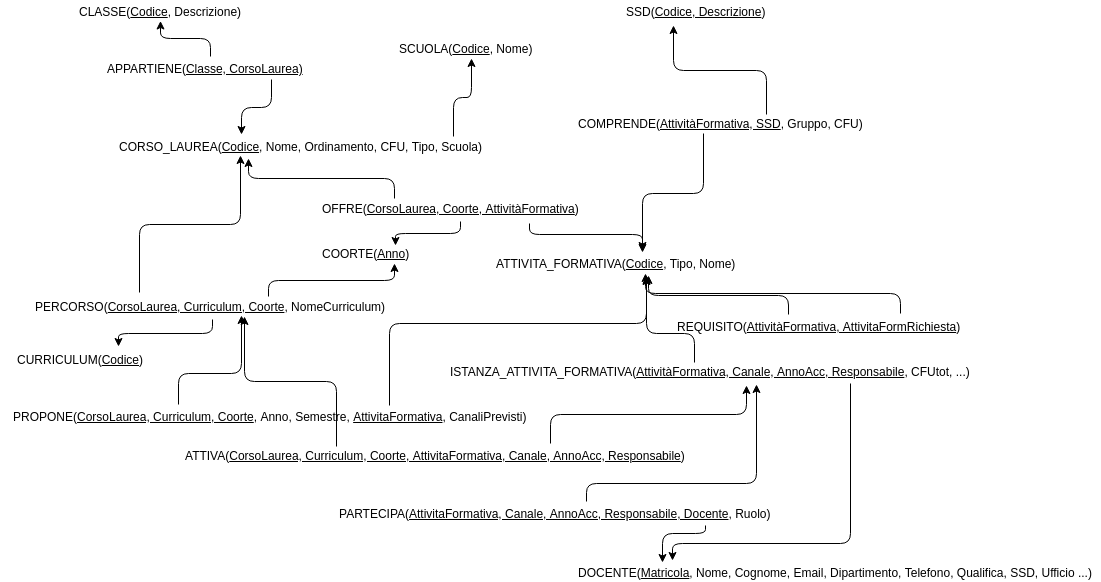
\includegraphics[scale=0.455,angle=90]{../Schemas/relational_model.jpg} %file va rinominato senza spazio senno viene plottato il nome file
	\end{center}
\end{figure}

\subsection{Schema logico e regole di vincolo}

\begin{itemize}
	\item RV1: i Corsi di Laurea devono essere proposti da una Scuola.
	\item RV2: i Corsi di Laurea devono appartenere ad una Classe.
	\item RV3: i Corsi di Laurea devono offrire almeno una Attivit\'a Formativa.
	\item RV4: i Percorsi devono proporre almeno una Attivit\'a Formativa.
	\item RV5: le istanze delle Attivit\'a Formative devono essere attivate per almeno un Percorso.
\end{itemize}

\newpage
% *****sezione4****
\section{SQL}



\subsection{Struttura}

\lstinputlisting[language=SQL]{../SQL/didactics.sql}

\subsection{Query}
\label{sql:query}

\lstinputlisting[language=SQL]{../SQL/interrogations.sql}
\newpage
% *****sezione 5*****

\section{Note}

Le frequenze delle operazioni non vengono riportate poic\'e non sono note.
Le regole di vincolo RV4, RV5 vengono implementate a livello applicativo utilizzando l'interrogazione proposta nella sezione \hyperref[sql:query]{query}.


% Uncomment the following two lines if you want to have a bibliography. Please do not forget to add an entry to your bibliography and reference it by using the \cite{} command
%\bibliographystyle{alphadin}
%\bibliography{document}

% End of the document
\end{document}